148. \begin{figure}[ht!]
\center{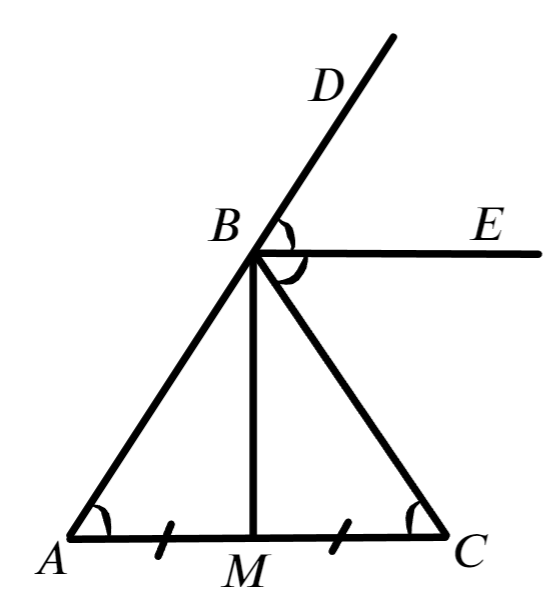
\includegraphics[scale=0.35]{g7-148.png}}
\end{figure}\\
Пусть $BE$ --- биссектриса внешнего угла, тогда $\angle DBE=\angle CBE.$ Так как по условию $BE\parallel AC,$ имеем равенства $\angle A=\angle DBE=\angle CBE=C$ (первые два угла равны как соответственные, вторые --- как накрест лежащие). Тогда треугольник $ABC$ является равнобедренным и его медиана $BM$ совпадает с высотой, поэтому $BM\perp AC,$ а значит и $BM\perp BE$ (так как $BE\parallel AC$). Поэтому угол между этой биссектрисой и медианой равен $90^\circ.$
ewpage
oindent
